
\chapter{太陽光発電データの時刻補正手法}
\label{chap:second}

\section{緒言}
本章では, 太陽光発電データの計測日時の補正手法を提案する.

% 20220523

\section{太陽光発電の計測データの問題点について}
本研究で管理している太陽光発電データは, データを計測しているPCの内部時計が標準時刻とずれているため, 他地点で計測しているデータと時刻同期ができない問題があった. 

そこで, 時刻がずれていない実測データと, 計算式により求まる大気外日射量との間の時間的遅延の秒数を相互相関を用いて求めることで, 実測データを標準時に補正する.

\section{大気外日射量の計算式}
任意の緯度経度, 日時における大気外日射量$Q$は, 任意の緯度$\phi$, 経度$\lambda$の地点における任意の日時, 太陽高度$\alpha$から求めることができる.

まず, 次式より元旦からの通し日数$dn$に基いて定めた$\theta$を用いて, 当該日の太陽赤緯$\delta$, 地心太陽距離$\frac{r}{r^{*}}$, 均時差$E_q$をそれぞれ以下の式により求める.
\begin{eqnarray}
  \theta =  \frac{2\pi (dn-1)}{365}
\end{eqnarray}

\begin{eqnarray}
  \begin{split}
    \delta =  0.006918-0.399912\cos \theta+0.070257\sin \theta-0.006758\cos 2\theta\\
    +0.000907\sin 2\theta-0.002697\cos 3\theta+0.001480\sin 3\theta
  \end{split}
\end{eqnarray}

\begin{dmath}
  \frac{r}{r^{*}} =  \frac{1}{\sqrt{1.000110+0.034221\cos \theta+0.001280\sin \theta+0.000719\cos 2\theta+0.000077\sin 2\theta}}
\end{dmath}

\begin{eqnarray}
  \begin{split}
    E_q =  0.000075+0.001868\cos \theta-0.032077\sin \theta\\
    -0.014615\cos 2\theta-0.040849\sin 2\theta
  \end{split}
\end{eqnarray}

日本標準時間から, 太陽の時角$h$を求める.

\begin{eqnarray}
  h = \frac{(日本標準時間-12)\pi}{12}+標準子午線からの経度差+E_q
\end{eqnarray}

$\delta$, $\phi$, $h$の値が既知となったので$\alpha$は

\begin{eqnarray}
  \alpha = \arcsin (\sin \phi\sin \delta+\cos \phi\cos \delta\cos h)
\end{eqnarray}

により求まる.

最後に, $Q$が

\begin{eqnarray}
  Q = 1367(\frac{r^{*}}{r})^{2}\sin \alpha
\end{eqnarray}

により求まる. 1367\si{\watt}/\si{\metre\squared}は太陽定数である.

式(2.1)~式(2.7)を用いることで, 任意の緯度経度, 日時における大気外日射量が求まる.

% 20220529

\subsection{実測データと大気外日射量との比較}
Elasticsearchサーバーから取得した2022年6月2日の実測データと, 計算式から求めた大気外日射量をプロットしたものを図\ref{20220529-p1}に示す. 実測データは地表に設置された太陽光パネルが計測したものであるのに対して, 大気外日射量は地球大気の上端(約8km上空)で受け取る日射量を計算したものであるため, 一日を通して最大となる日射量の大きさに差がある.

\begin{figure}[H]
  \begin{center}
    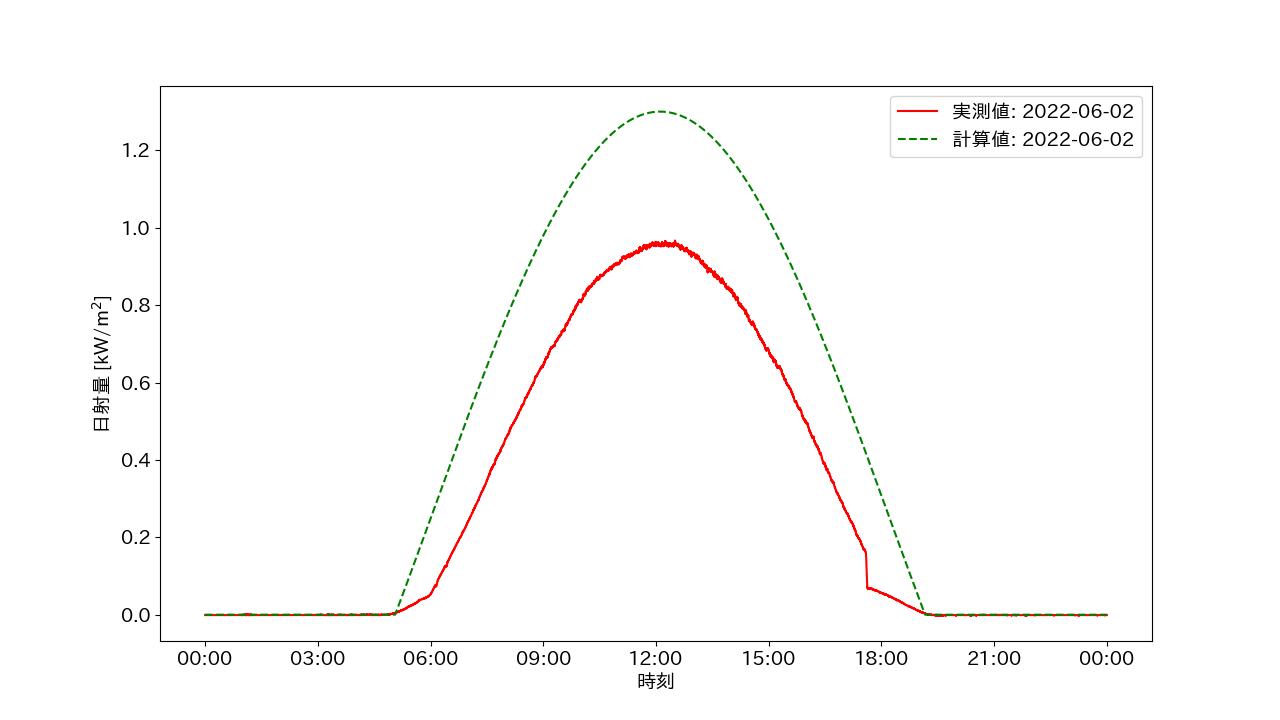
\includegraphics[width=160mm]{sotu/figure/2/original-20220602-corr.png}
    \caption{2022年6月2日の日射量の実測データと大気外日射量をプロットしたもの}
    \label{20220529-p1}
  \end{center}
\end{figure}

% 20220620

\subsection{相互相関による時刻補正法}
今回, 相互相関の計算に使用する期間を, 2022年6月2日0時0分から2022年6月2日23時59分までとする.

% 2022年6月2日を選定した理由は, 図\ref{20220529-p1}より, 2022年6月2日の実測データの概形は大気外日射量の概形と類似していたためである.

相互相関の計算に使用する実測データの計測日時から大気外日射量を求め, 実測データとの相互相関を計算する.

相互相関を計算した結果, 実測データを124秒遅らせた際に, 相関が最大となった.

今回使用した実測データには計測日時のずれは殆どないため, 実測データを遅らせていない際に相関が最大となるのが正しい.

これは, 相互相関を計算する際に地表日射量ではなく大気外日射量を使用していることが原因であると考えられる.

\section{地表日射量の予測}

地表日射量の予測を行うため, 式(2.1)~式(2.7)を使った方法ではなく, pvlibライブラリを使用して地表日射量を求め, 相互相関を計算する.

\subsection{pvlibの概要}
pvlibは, 太陽光発電システムの性能シミュレーションや関連するタスクを実行するための関数とクラスのセットを提供するライブラリである. 

以下は, pvlibの主な特徴である.

\begin{itemize}
  \item 太陽位置計算: pvlibは, 地球上の任意の場所における太陽の位置を計算する機能を提供する. これは, 太陽の方位角や高度角を求めるのに使用される.
  \item 大気透過モデル: 大気を通過する太陽放射の量や質を推定するモデルが含まれている.
  \item 太陽光発電システムの性能モデリング: 太陽光発電モジュールやインバーターの性能モデルが含まれており, 異なる条件下での太陽光発電システムの出力をシミュレートできる.
\end{itemize}

\subsection{実測データとpvlibにより求まる地表日射量の比較}
Elasticsearchサーバーから取得した実測データと, pvlibを用いて求めた地表日射量をプロットしたものを図\ref{2-p1}に示す.
% 図\ref{2-p1}はElasticsearchサーバーから取得した2022年6月2日の日射量データと, リサイクル館の緯度経度と日付情報を入力としてpvlibより求めた地表日射量をプロットしている.

図\ref{2-p1}と図\ref{20220529-p1}と比較すると, 大気外日射量より地表日射量の方が実測データにより近い概形となっていることが分かる.

\begin{figure}[H]
  \begin{center}
    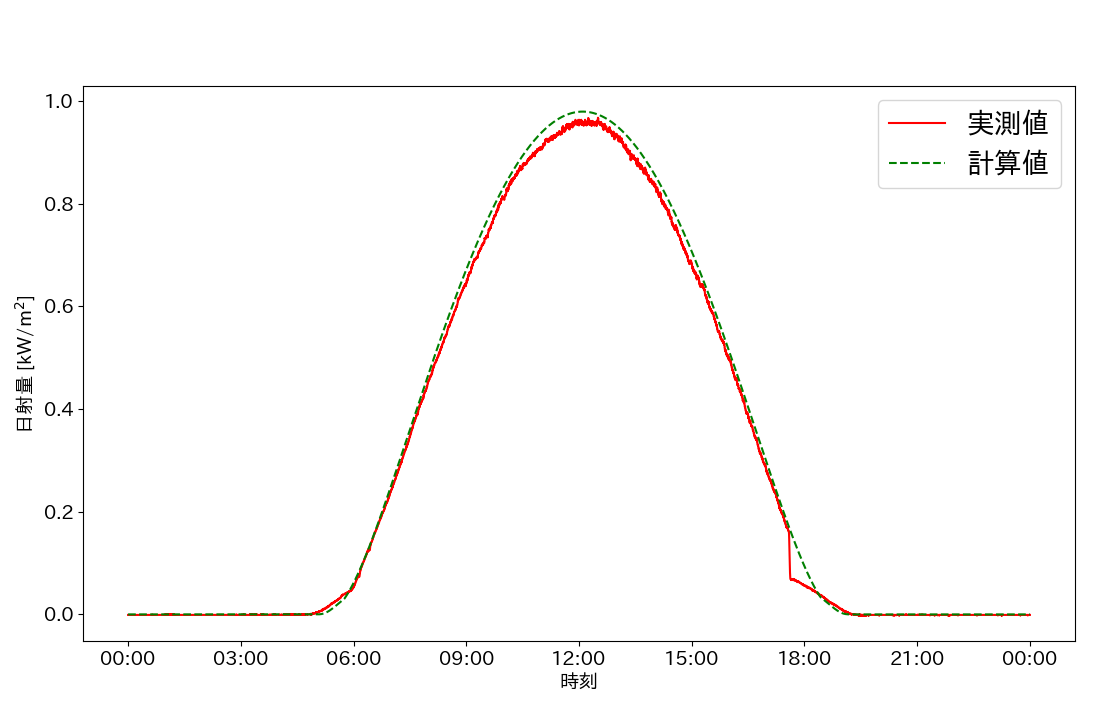
\includegraphics[width=160mm]{sotu/figure/2/pvlib-20220602-corr.png}
    \caption{2022年6月2日の実測データと地表日射量をプロットしたもの}
    \label{2-p1}
  \end{center}
\end{figure}

\subsection{地表日射量との相互相関による時刻補正法}
今回, 相互相関の計算に使用する期間を, 2022年6月2日0時0分から2022年6月2日23時59分までとする.

実測データの計測日時から地表日射量を求め, これらの値から相互相関を計算する.

相互相関を求めた結果, 実測データ74秒遅らせた際に, 相関が最大となることが分かった.

式(2.1)~式(2.7)より求めた大気外日射量を用いて相互相関を計算した時と比較して, 124秒から74秒へと50秒改善した.

\section{前処理の追加による時刻補正法とその精度}

図\ref{2-p1}では, 日没の辺りにおいて, 実測データと地表日射量の概形が大きく異なっている.

太陽光パネルの周囲にある建造物や, 天候といった外部要因による実測データのひずみを事前に取り除いた上で相互相関を計算することで, 相互相関の計算結果が改善するか検証する. そこで, 実測データに対して前処理を追加する.

前処理を含めた相互相関の計算方法は以下の手順で行う.

\begin{enumerate}
  \item 実測データの日射量を0 \si{\kilo\watt}/\si{\metre\squared}と見なすしきい値の指定: まず, 実測データをフィルタリングするために日射量のしきい値を設定する. 今回は, 0.2 \si{\kilo\watt}/\si{\metre\squared}をしきい値として設定する.
  \item しきい値に該当する計測日時の特定: 続いて, 実測データの各データ点から0.2 \si{\kilo\watt}/\si{\metre\squared}を減算して絶対値を取った際に最も0に近い値を取る計測日時を午前と午後でそれぞれ一点ずつ特定する.
  \item 特定した計測日時を使った実測データのフィルタリング: 前のステップで得た計測日時を使用して, 2点の計測日時の外側にある実測データの日射量を0 \si{\kilo\watt}/\si{\metre\squared}とする.
  \item 地表日射量との相互相関の計算: 実測データをフィルタリングした後, 地表日射量との相互相関を計算する.
\end{enumerate}

図\ref{2-p2}に, 上述の前処理を行った実測データと, 地表日射量をプロットしたものを示す.

\begin{figure}[H]
  \begin{center}
    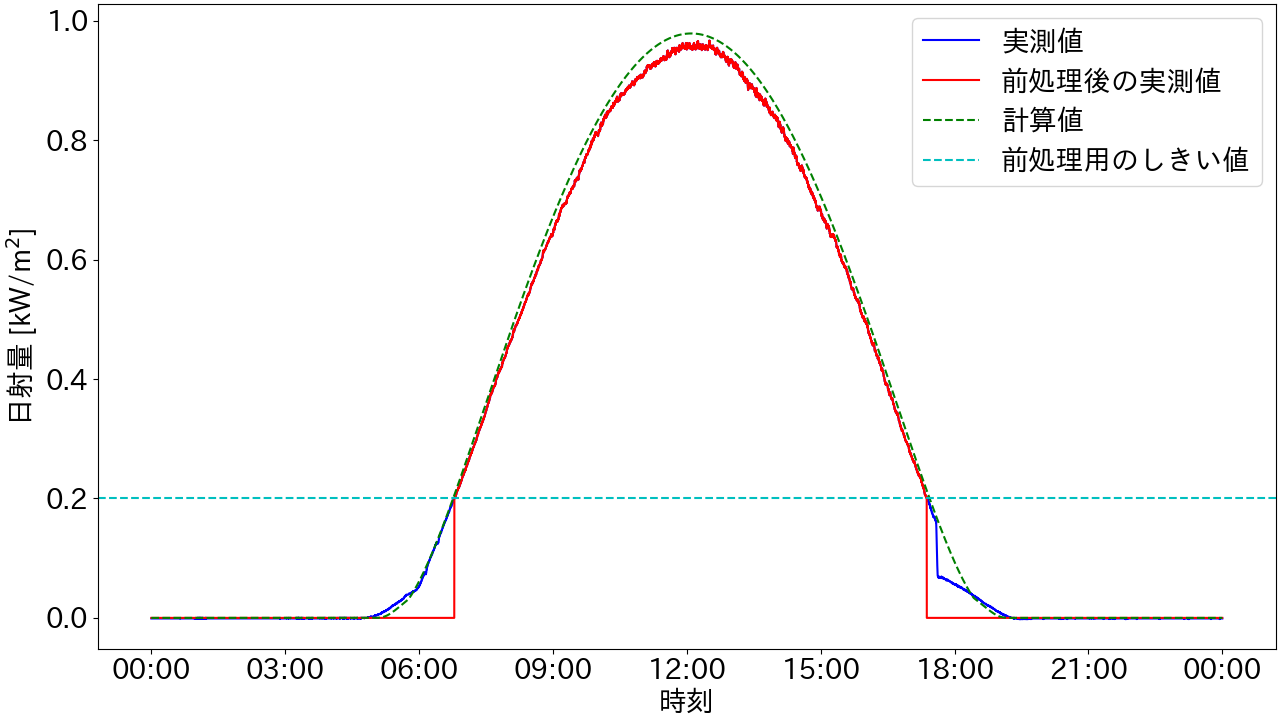
\includegraphics[width=140mm]{sotu/figure/2/drop-under-0.2-q.png}
    \caption{前処理を行った実測データと, 地表日射量をプロットしたもの}
    \label{2-p2}
  \end{center}
\end{figure}

前処理を行った実測データと, 地表日射量から相互相関を計算した結果, 実測データを27秒遅らせた際に, 相関が最大となった.

前処理を追加したことで相互相関の結果が, 74秒から27秒へと47秒改善した.

\section{結言}
本章では太陽光発電データの計測時刻の補正手法を提案した.
次章では学内ゾーンで稼働している Elasticsearch クラスタへのデータ移行について述べる.